%%%%%%%%%%%%%%%%%%%%%%%%%%%%%%%%%%%%%%%%%
% Stylish Article
% LaTeX Template
% Version 2.1 (1/10/15)
%
% This template has been downloaded from:
% http://www.LaTeXTemplates.com
%
% Original author:
% Mathias Legrand (legrand.mathias@gmail.com) 
% With extensive modifications by:
% Vel(vel@latextemplates.com)
%
% License:
% CC BY-NC-SA 3.0 (http://creativecommons.org/licenses/by-nc-sa/3.0/)
%
%%%%%%%%%%%%%%%%%%%%%%%%%%%%%%%%%%%%%%%%%

%----------------------------------------------------------------------------------------
%	PACKAGES AND OTHER DOCUMENT CONFIGURATIONS
%----------------------------------------------------------------------------------------

\documentclass[fleqn,10pt]{JLA_article} % Document font size and equations flushed left

\usepackage[english]{babel} % Specify a different language here - english by default

\usepackage{lipsum} % Required to insert dummy text. To be removed otherwise


%----------------------------------------------------------------------------------------
%	HYPERLINKS
%----------------------------------------------------------------------------------------

\usepackage{hyperref} % Required for hyperlinks
\hypersetup{hidelinks,colorlinks,breaklinks=true,urlcolor=color2,citecolor=color1,linkcolor=color1,bookmarksopen=false,pdftitle={Title},pdfauthor={Author}}

%----------------------------------------------------------------------------------------
%	ARTICLE INFORMATION
%----------------------------------------------------------------------------------------

\PaperTitle{JLA Article Template} % Article title

\Authors{John Smith\textsuperscript{1}*, James Smith\textsuperscript{2}} % Authors
\affiliation{\textsuperscript{1}\textit{Department of Education, Example University, City, Country. email icon: somebody@gmail.com}} % Author affiliation
\affiliation{\textsuperscript{2}\textit{Department of Computer Science, Example University, City, Country. email icon: somebody@gmail.com}} % Author affiliation

\Keywords{Include a set of keywords related to your submission. Separate them by commas.} 

\Submitted{10/11/12}
\Accepted{10/11/12}
\Published{10/11/12}

\Volume{1}
\Number{1}
\Pages{1---10}
\Doi{xxx-xxx-xxx}
%----------------------------------------------------------------------------------------
%	NOTES FOR PRACTICE OR RESEARCH
%----------------------------------------------------------------------------------------
%\WithoutNotestrue %If this paper does NOT have notes
\Notesname{Notes for Practice} %If this is a Research Paper
%\Notesname{Notes for Research} %If this is a Practitioner Paper


\note{This is an example of a note to practice or research.}
\note{This is a second example of a note to practice or research.}
\note{This is a third example of a note to practice or research.} %Add more notes if necesary

%----------------------------------------------------------------------------------------
%	ABSTRACT
%----------------------------------------------------------------------------------------

\Abstract{Abstracts shall not exceed 200 words. Do not use a heading for the abstract or headings within the abstract.\\ \lipsum[1]~}

%----------------------------------------------------------------------------------------

\begin{document}

\flushbottom % Makes all text pages the same height

\maketitle % Print the title and abstract box

%\tableofcontents % Print the contents section

\thispagestyle{fancy} % Add header to first page


%----------------------------------------------------------------------------------------
%	ARTICLE CONTENTS
%----------------------------------------------------------------------------------------

\section{Introduction} % The \section*{} command stops section numbering

\addcontentsline{toc}{section}{Introduction} % Adds this section to the table of contents

This is example text. Note that JLA uses up to 3 levels of headings (e.g. 1., 1.1, 1.1.1). Please do not add additional levels beyond the three that have been provided. This is an example of including math $\cos\pi=-1$ and $\alpha$ directly within the text\footnote{And an example of a footnote including math $\cos\pi=-1$ and $\alpha$ in the text.}. Important formulas should be presented on a seperate line as shown in the next section (See Formula 1). All figures and tables should be explicitly referenced in the appropriate part of the text (See Table 1 and Figure 2).

This template use the  \href{http://ctan.uniminuto.edu/biblio/bibtex/contrib/apacite/apacite.pdf}{apacite package}. This is an example on how to cite \cite{Figueredo:2009dg}.  Here is a citation when you want to address the authors directly, for example the work of \citeA{archambault2009student}.


\lipsum[1] % Dummy text

%------------------------------------------------

\section{Literature Review}

\lipsum[2-3] % Dummy text

%------------------------------------------------

\section{Methods}

\begin{figure}[ht]\centering % Using \begin{figure*} makes the figure take up the entire width of the page
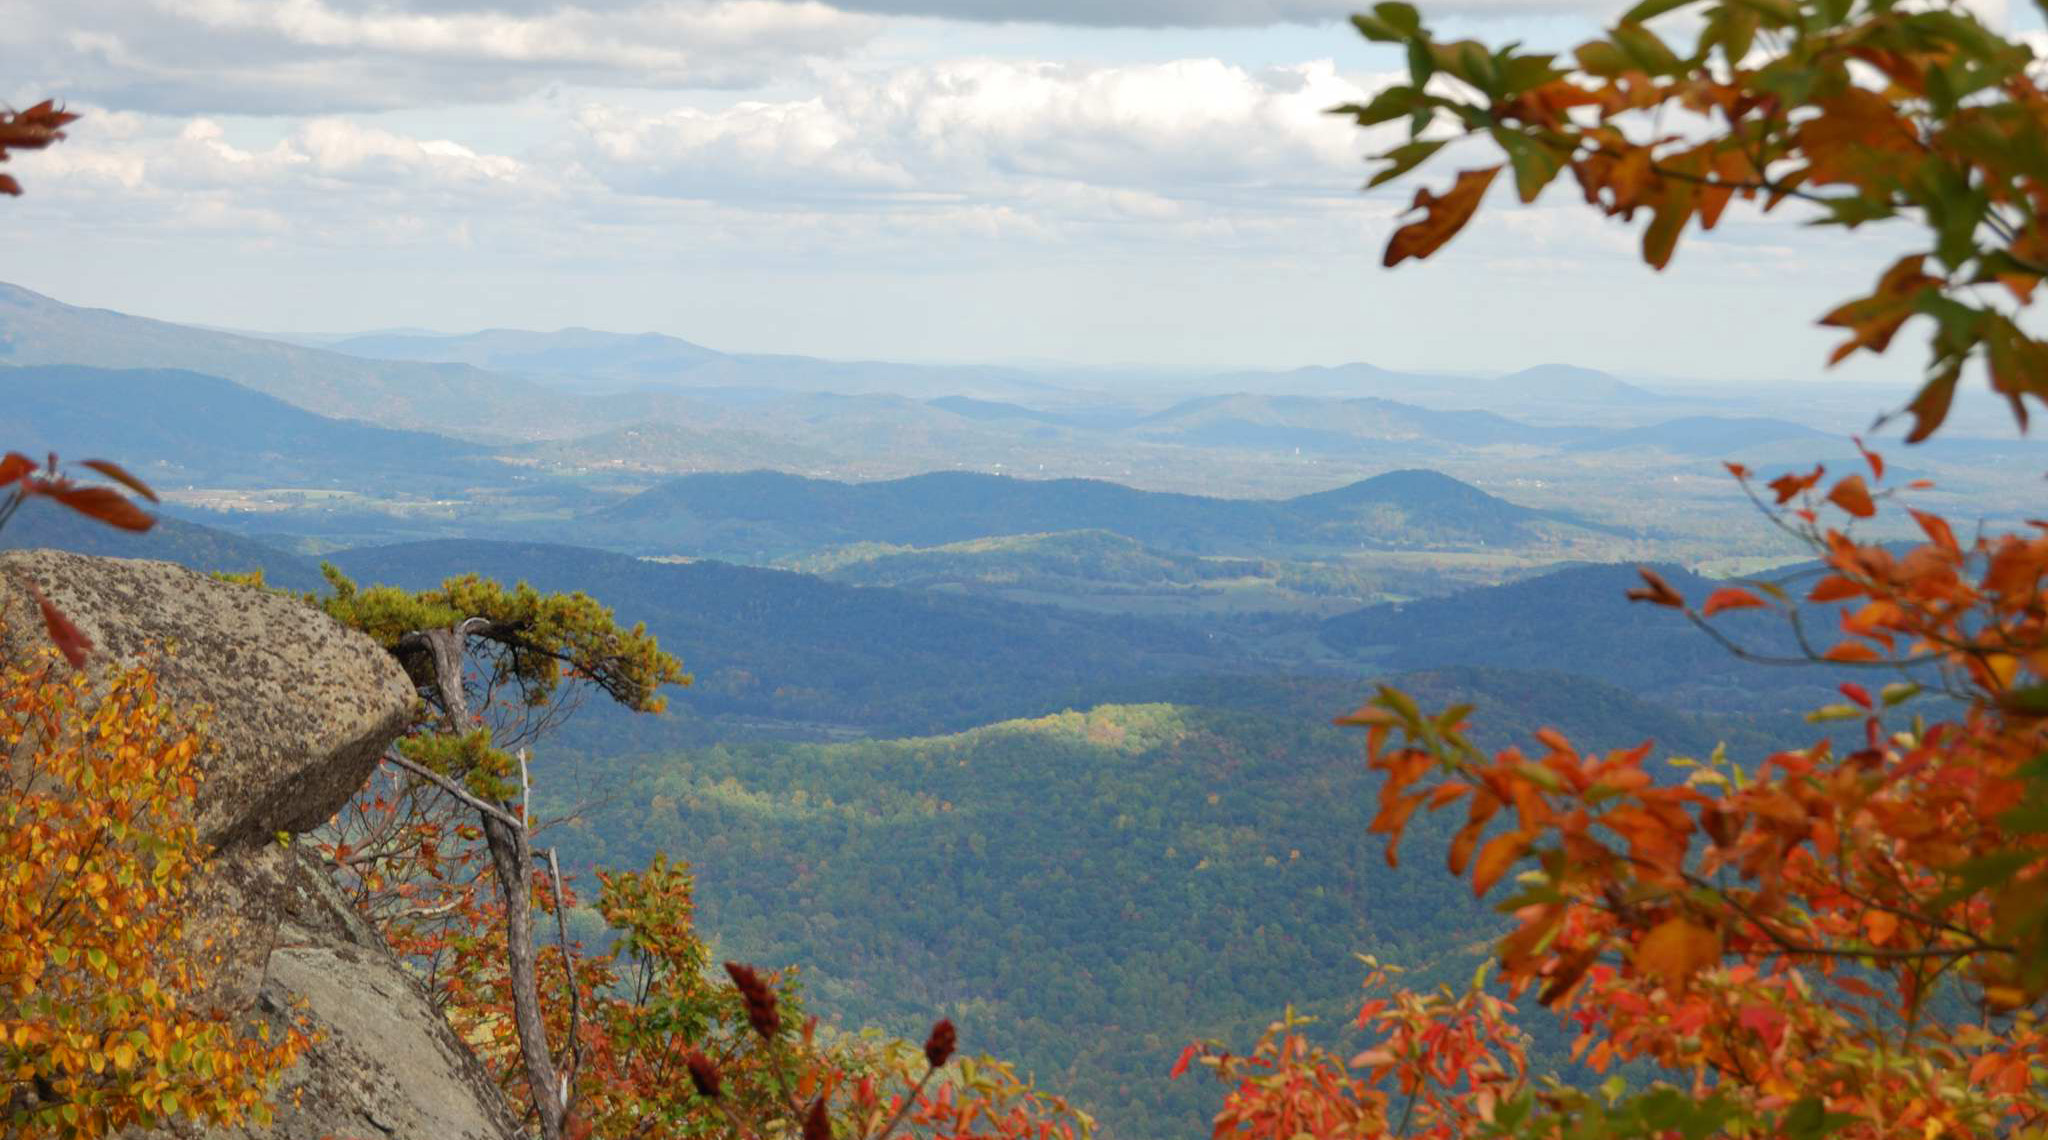
\includegraphics[width=\linewidth/2]{view}
\caption{Picture}
\label{fig:view}
\end{figure}

\lipsum[4] % Dummy text

\begin{equation}
\cos^3 \theta =\frac{1}{4}\cos\theta+\frac{3}{4}\cos 3\theta
\label{eq:refname2}
\end{equation}

\lipsum[5] % Dummy text

\begin{enumerate}[noitemsep] % [noitemsep] removes whitespace between the items for a compact look
\item First item in a list
\item Second item in a list
\item Third item in a list
\end{enumerate}

\subsection{Subsection}

\lipsum[6] % Dummy text

%\paragraph{Paragraph} \lipsum[7] % Dummy text
%\paragraph{Paragraph} \lipsum[8] % Dummy text

\subsection{Subsection}

\lipsum[9] % Dummy text

\begin{figure}[ht]\centering
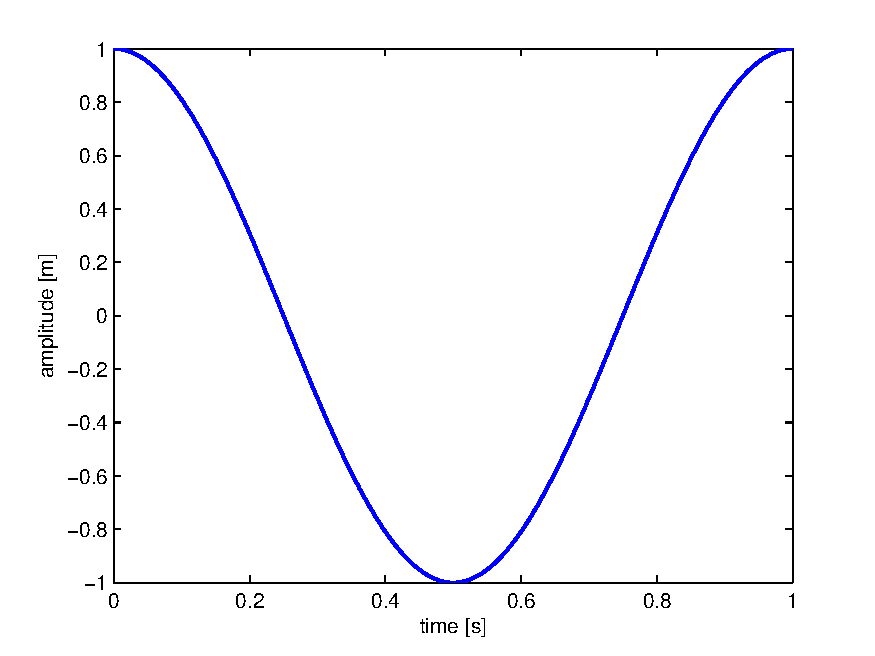
\includegraphics[width=\linewidth/2]{results}
\caption{In-text Picture}
\label{fig:results}
\end{figure}

Reference to Figure \ref{fig:results}.

%------------------------------------------------

\section{Results and Discussion}

\lipsum[10] % Dummy text

\subsection{Subsection}

\lipsum[11] % Dummy text

\begin{table}[hbt]
\caption{Table of Grades}
\centering
\begin{tabular}{llr}
\toprule
\multicolumn{2}{c}{Name} \\
\cmidrule(r){1-2}
First name & Last Name & Grade \\
\midrule
John & Doe & $7.5$ \\
Richard & Miles & $2$ \\
\bottomrule
\end{tabular}
\label{tab:label}
\end{table}

\subsubsection{Subsubsection}

\lipsum[12] % Dummy text

\begin{description}
\item[Word] Definition
\item[Concept] Explanation
\item[Idea] Text
\end{description}

\subsubsection{Subsubsection}

\lipsum[13] % Dummy text

\begin{itemize}[noitemsep] % [noitemsep] removes whitespace between the items for a compact look
\item First item in a list
\item Second item in a list
\item Third item in a list
\end{itemize}

\subsubsection{Subsubsection}

\lipsum[14] % Dummy text

\section{Conclusion}

\lipsum[15] % Dummy text

%------------------------------------------------
\phantomsection
\section*{Acknowledgments} % The \section*{} command stops section numbering
\addcontentsline{toc}{section}{Acknowledgments} % Adds this section to the table of contents

To the creators of  \LaTeX.


\section*{Declaration of Conflicting Interest} % The \section*{} command stops section numbering

\addcontentsline{toc}{section}{Declaration of Conflicting Interest} % Adds this section to the table of contents

The author(s) declared no potential conflicts of interest with respect to the research, authorship, and/or publication of this article.

\section*{Funding} % The \section*{} command stops section numbering

\addcontentsline{toc}{section}{Funding} % Adds this section to the table of contents

This study was financially supported by Company X.

%----------------------------------------------------------------------------------------
%	REFERENCE LIST
%----------------------------------------------------------------------------------------
\phantomsection
\bibliography{sample}

%----------------------------------------------------------------------------------------

\end{document}